\documentclass[esp]{ECCI-SIME-class}
% Título del Articulo
\title{Sistema de reconocimiento facial por IA}
\shorttitle{- Seminario Internacional-}

% Autores
\author[1]{Jorge Ivan Torres Florez}
\author[2]{Cristan David Parra Torres}
\author[3]{Juan Camilo Morales Sierra}

% Información de los autores
\affil[1]{jorgei.torresf@ecci.edu.co, Ingenieria Electronica}
\affil[2]{cristiand.parrat@ecci.edu.co, Ingenieria Electronica}
\affil[2]{juanc.moraless@ecci.edu.co, Ingenieria Electronica}

 % Iniciar documento
\begin{document}

% Introduzca el resumen en español
\resumen{
El presente informe detalla el desarrollo del reto solicitado para el seminario, un sistema de reconocimiento facial basado en inteligencia artificial, haciendo uso de librerias varias, entre la mas desacada OpenCV, una Raspberry Pi Zero 2w y una camara para la detección de rostros.}

% Introduzca las palabras clave en español 
\palabrasclave{
RECONOCIMINETO FACIAL, OPENCV, RASPBERRYPI, IA
}

% Insert here the abstract in English language
\abstract{
\textit{
This report details the development of the challenge requested for the seminar, a facial recognition system based on artificial intelligence, using several libraries, among the most notable OpenCV, a Raspberry Pi Zero 2w and a camera for face detection.
} }

% Insert here the keywords of your work in English language
\keywords{
 \textit{
FACIAL RECOGNITION, OPENCV, RASPBERRYPI, IA.}
}

\maketitle
\thispagestyle{fancy}

\section{1.	INTRODUCCIÓN} 

La seguridad y el control de accesibilidad ha evolucionado durante estos últimos años, presentando nuevas metodologías y desarrollos para el avance de sistemas de seguridad tales como, el reconocimiento facial siendo una de las aplicaciones más avanzadas y utilizadas de la inteligencia artificial en estos momentos. Con la implementación de la IA y tecnologías nuevas, es posible el desarrollo de sistemas de reconocimiento facial de bajo costo y consumo energético, como en este caso la Raspberry Pi.

El objetivo con este proyecto es el desarrollo de un sistema de reconocimiento facial, usando como medio una raspberry pi Zero 2w, librerías diversas como OpenCV y una cámara. Mediante el uso de modelos de aprendizaje, buscando el optimizar lo mayor posible, para el reconocimiento de rostros en tiempo real, garantizando un resultado fiable incluso en situaciones de poca o mucha luminosidad o ángulos de captura.

A lo largo de este informe, se tocaran temas como aspectos técnicos relacionados con la instalación y configuración de los dispositivos, así como la elección del sistema de aprendizaje más adecuado para el reconocimiento facial, se analizaran los resultados obtenidos en pruebas con distintas condiciones de exposición, buscando las mayor optimización y reconocimiento por parte del sistema para futuras versiones.

Se realizara una demostración de como realizar las capturas de las imagenes, el modelo y la identificación de los distintos rostros de las personas

\section{2.	METODOLOGÍA}
El proyecto se centra en el desarrollo de un sistema automatizado de reconocimiento facial mediante una camara donde reconoce a la persona y valida si es autorizada o denegada utilizando inteligencia artificial. Adicionalmente se va a dar una explicación general sobre el reconocimiento facial en Python con OpenCV.
 \\

\begin{figure}[!h] 
     \centering
     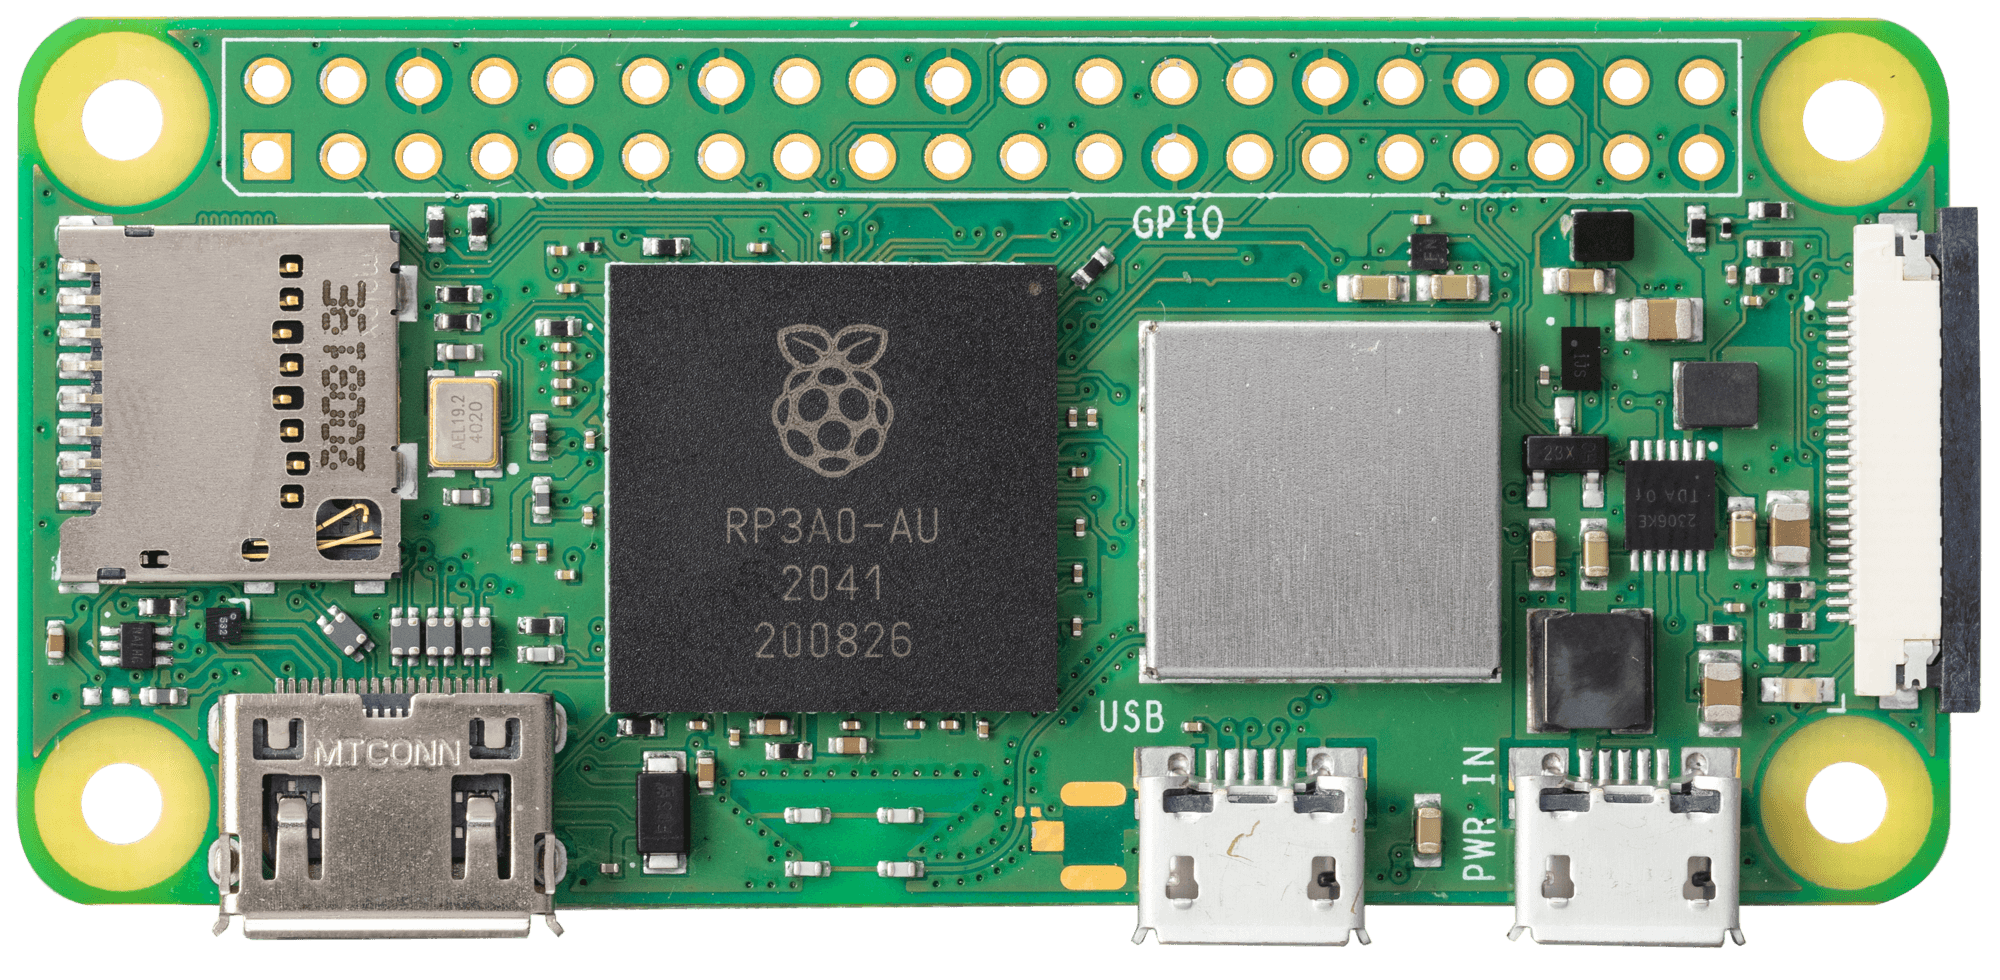
\includegraphics[width=.8\columnwidth]{Plantilla IEEE ECCI/Imagenes/zero2-close-up.png} 
     \caption{Raspberry Pi Zero 2W} \label{fig-1}
\end{figure} 

\\Actúa como la unidad central de procesamiento y control del sistema. La Raspberry Pi puede ejecutar programas complejos, manejar la interfaz de usuario, y coordinar la comunicación entre los diferentes componentes.
Ventajas: Su capacidad de conectividad (Wi-Fi, Bluetooth), posibilidad de programación en varios lenguajes y soporte para múltiples interfaces de entrada/salida. \\ \\


\section{3.	RESULTADOS Y DISCUSIÓN}

Para poner en marcha un sólido sistema de reconocimiento facial basado en Python y OpenCV, siga un procedimiento organizado de tres etapas. Primero, desarrolle un conjunto de datos etiquetados que contenga entre 20 y 30 imágenes faciales en escala de grises por individuo mediante una cámara web, utilizando Haar Cascades para la identificación de rostros en tiempo real y las herramientas de preprocesamiento de OpenCV (como la ecualización de histograma, la modificación del tamaño a 100 × 100 píxeles). Elabore imágenes en directorios de asuntos concretos para acelerar la formación. Seguidamente, entrene un modelo LBPH (histogramas de patrones binarios locales) empleando cv2, que codifica patrones de textura exclusivos para cada cara en un archivo.yml que puede ser reutilizado. Verifique la exactitud del modelo mediante un conjunto de ensayos de reserva.


\section{3.	DISEÑO EXPERIMENTAL}
Realizamos el montaje de un sistema controlado , compuesto por una galga y un encoder como base de control. 

\section{3.1Objetivo del Proyecto:}

Demostrar el funcionamiento de un agitador en un líquido newtoniano y su impacto en el esfuerzo del motor según la cantidad de líquido vertido.

\section{Descripción: Preparación Inicial:} El contenedor del líquido debe estar completamente vacío antes de comenzar el experimento.

\textbf{Adición de Líquido:} Se va a verter una mezcla de agua y fécula de maíz, que actúa como un líquido newtoniano, en el contenedor.
\textbf{Operación del Agitador:}El agitador debe comenzar a girar una vez que el líquido esté en el contenedor. 
\textbf{Observación del Esfuerzo del Motor:}A medida que se añade más líquido, se observará que el motor necesita realizar un esfuerzo mayor para mantener la velocidad de giro en el valor deseado (set point).
\textbf{Meta: }Evaluar cómo la densidad y el volumen del líquido afectan la carga del motor y la capacidad del sistema para mantener la velocidad de giro establecida.

\textbf{Indicadores de Éxito:}

- El agitador debe poder girar en el líquido inicial sin dificultad.
- Se debe notar un incremento en el esfuerzo del motor proporcional al aumento de líquido.
- El sistema debe ser capaz de ajustar y mantener la velocidad de giro deseada, aunque el esfuerzo del motor varíe.



\section{3. RESULTADOS }

Señal del Encoder:

En el osciloscopio, verás una serie de pulsos cuadrados que corresponden a la rotación del agitador. Si el agitador está girando a 2 vueltas por segundo y el encoder genera 10 pulsos por vuelta, verás 20 pulsos por segundo en la pantalla del osciloscopio.
La distancia entre los pulsos debe ser uniforme si la velocidad del agitador es constante.
Señal PWM:

La señal PWM aparece como una onda cuadrada en la pantalla del osciloscopio. A 2 vueltas por segundo, el ciclo de trabajo del PWM ajustará la potencia entregada al motor para mantener esta velocidad.
Un ciclo de trabajo alto (más tiempo en estado alto) indica que se está suministrando más potencia al motor, mientras que un ciclo de trabajo bajo (más tiempo en estado bajo) indica menos potencia.
En la pantalla del osciloscopio, notarás que la frecuencia de la señal PWM es mucho más alta que la frecuencia de los pulsos del encoder. La forma de onda mostrará los cambios en el ciclo de trabajo que corresponden al esfuerzo del motor para mantener la velocidad de 2 vueltas por segundo.




\section{3.1.  Implementación del Convertidor de 4 a 20 mA y Control del Batidor}


Para lograrlo, se implementó un convertidor de 4 a 20 mA utilizando un amplificador operacional LM741, se midió el nivel de agua y se controló la velocidad del batidor. Además, se utilizó un amplificador instrumental AD620 para amplificar la señal de una galga extensiométrica, mejorando la precisión y sensibilidad de las mediciones.

Implementación Técnica
1. Amplificación de Señal con AD620:

Propósito: Mejorar la precisión de la medición del nivel de agua mediante la amplificación de la señal de la galga extensiométrica.

Componentes:

AD620: Amplificador instrumental de alta precisión utilizado para amplificar la pequeña señal de la galga extensiométrica se calculo una resistencia de ganacia de 10ohms .
Galgas Extensiométricas: Sensores que miden la deformación (strain) y proporcionan una señal de voltaje proporcional a la fuerza aplicada, que en este caso está relacionada con el nivel de agua. 

La galga extensiométrica detecta la deformación causada por el nivel de agua en el contenedor y produce una señal de voltaje muy pequeña.
El AD620 amplifica esta señal para que pueda ser procesada de manera efectiva por el sistema de control.
La ganancia del AD620 se ajusta según las necesidades del proyecto para asegurar que la señal amplificada esté dentro del rango adecuado para el convertidor de 4 a 20 mA.
2. Convertidor de 4 a 20 mA:

Propósito: Convertir la señal amplificada de la galga extensiométrica en una corriente estándar de 4 a 20 mA.
Componentes:
LM741: Amplificador operacional utilizado para procesar la señal amplificada del AD620 y ajustar la corriente de salida.
Circuito Básico:
La señal amplificada por el AD620 se alimenta al LM741.
El LM741 se configura para convertir esta señal de voltaje en una corriente de 4 a 20 mA.
A un nivel bajo de agua, la salida del circuito es 4 mA.
A un nivel alto de agua, la salida del circuito es 20 mA.
3. Medición del Nivel de Agua:

Proceso:
La señal amplificada de la galga extensiométrica, que ahora es lo suficientemente fuerte y precisa, se convierte en una señal de corriente de 4 a 20 mA mediante el LM741.
Esta señal de corriente se utiliza para indicar el nivel de agua en el contenedor.
4. Control de la Velocidad del Batidor: \\

Interfaz con el Motor:

La señal de 4 a 20 mA se utiliza para controlar un variador de frecuencia o un controlador de motor, ajustando la velocidad del batidor.
La velocidad del batidor se ajusta dinámicamente según la señal de corriente, que corresponde al nivel de agua.
Funcionamiento: \\

A un nivel bajo de agua (4 mA), el batidor opera a una velocidad mínima.
A medida que el nivel de agua aumenta (hasta 20 mA), el batidor incrementa su velocidad para asegurar una mezcla adecuada.
Esto permite una respuesta dinámica del sistema, ajustando la velocidad del batidor en función del nivel de agua para mantener una mezcla homogénea.
Visualización y Resultados
En el Osciloscopio:

Señal del Convertidor:\\

La corriente de 4 a 20 mA muestra una relación lineal con el nivel de agua, gracias a la amplificación precisa del AD620.
La señal de corriente debería aumentar linealmente con el aumento del nivel de agua, reflejando la mejora en precisión por el AD620.
Control del Motor: \\

La señal de corriente de 4 a 20 mA se convierte en una señal de control para el variador de frecuencia del motor del batidor.
En el osciloscopio, se observará cómo el ciclo de trabajo del PWM (utilizado para controlar el motor) cambia en respuesta a la señal de 4 a 20 mA, ajustando la velocidad del batidor. \\


\section{7.	CONCLUSIONES}
\begin{itemize}
\item 
Precisión en el Control de Velocidad: La utilización de un encoder permite una medición precisa de las RPM de un motor o eje, lo que facilita un control fino y preciso de la velocidad. Esto es crucial en aplicaciones donde se requiere un funcionamiento estable y consistente, como en sistemas de transporte, maquinaria industrial o robótica.
\end{itemize}
\begin{itemize}
\item 
Mejora en la Productividad y Seguridad: Un control más preciso de las RPM mediante el uso del encoder y la visualización en un osciloscopio puede mejorar la productividad al reducir el tiempo de inactividad debido a problemas mecánicos.
\end{itemize}
\begin{itemize}
\item 
La adición del amplificador instrumental AD620 para amplificar la señal de la galga extensiométrica mejoró significativamente la precisión y sensibilidad del sistema de medición. Combinado con el convertidor de 4 a 20 mA y el LM741, permitió una medición precisa del nivel de agua y un control eficiente de la velocidad del batidor. Esta configuración asegura que el batidor opere a la velocidad óptima según el nivel de líquido, manteniendo la consistencia y calidad de la mezcla. El uso de estas tecnologías proporciona una solución robusta y confiable para el manejo del agitador en aplicaciones industriales.

\end{itemize}
\nocite{*}
\printbibliography
\end{document}
